\documentclass[%
 %superscriptaddress,
%groupedaddress,
%unsortedaddress,
%runinaddress,
%frontmatterverbose, 
%preprint,
%showpacs,preprintnumbers,
%nofootinbib,
%nobibnotes,
%bibnotes,
 amsmath,amssymb,
%aps,
%pra,
%prb,
%rmp,
%prstab,
%prstper,
%floatfix,
]{article}

\usepackage{graphicx}% Include figure files
\usepackage{dcolumn}% Align table columns on decimal point
\usepackage{bm}% bold math
\usepackage{hyperref}% add hypertext capabilities
\usepackage[mathlines]{lineno}% Enable numbering of text and display math
%\linenumbers\relax % Commence numbering lines

%\usepackage[showframe,%Uncomment any one of the following lines to test 
%%scale=0.7, marginratio={1:1, 2:3}, ignoreall,% default settings
%%text={7in,10in},centering,
%%margin=1.5in,
%%total={6.5in,8.75in}, top=1.2in, left=0.9in, includefoot,
%%height=10in,a5paper,hmargin={3cm,0.8in},
%]{geometry}
%\usepackage{biblatex}

\begin{document}

\title{Radiation and the fear factor}


\author{Nirupama Sensharma}

\date{\today}
%
\maketitle
%
%
% Some keywords, using a new command: \KeyWords{}
%

If I start by saying that Radiation is not dangerous, I would be lying. At the slightest mention of the R-word, most people get disturbing images of nuclear bombs, mushroom clouds and nuclear power plants in front of their eyes. While this is not entirely wrong, there is still a lot more to it. And, it is now high-time that every sane mind on the planet Earth knows what exactly is radiation.

The omniscient Google puts it as \textit{“\textbf{radiation} is the emission or transmission of energy in the form of  waves or particles through space.”} And if you dig a little deeper, you will find a list of all the different kinds of radiation. If you have not already, a quick tour of the Wiki page will tell you that in addition to the well known alpha ($\alpha$), beta ($\beta$) and gamma ($\gamma$) rays; radio waves, microwaves, X-rays, Visible light are all forms of radiation. However, we never worry about any exposure that we receive by say sitting under a light bulb for 12 hours or listening to radio all night long or heating our food in a microwave. The reason is because there is a subcategory that any kind of radiation can be divided into – ionizing and non-ionizing. Radiation like $\alpha$- $\beta$- $\gamma$- rays and X-rays that can possibly do harm to living tissues by ionizing atoms or knocking off electrons from atoms are ionizing. Whereas, radio waves, microwaves and Visible light that are on the lower frequency end of the Electromagnetic spectrum, cannot ionize atoms and are unable to cause any potential damage to the living tissues are non-ionizing radiation.

\begin{figure}
\begin{center}
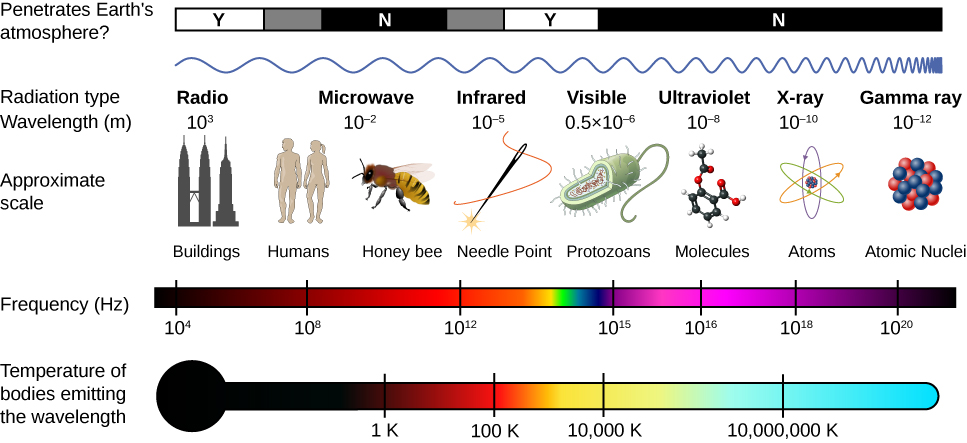
\includegraphics[width = \textwidth]{EM_spectrum}
\caption{The level scheme of $^{135}Pr$ as given in. Clearly labeled are the Yrast, wobbling, Dipole and the Signature partner bands.}
\end{center}
\end{figure}

The first nuclear explosion was the Trinity nuclear test conducted as a part of the Manhattan Project by the US back in 1945 and the first nuclear power plant to be connected to the power grid was in Obninsk, Russia in the year 1954. So can it be safely said that the Radiation exposure problem started only after these events? Well, the answer is a clear No!

Radiation has been a part of human life since the beginning of time. The radiation as emitted by nuclear explosions and reactors or more commonly referred to as the man-made radiation sources is always made a big agenda. However, it is not very well known that in addition to the man-made sources of radiation, there is also an appreciable contribution from the natural sources of radiation. 

The dose as received from the natural sources of radiation are often termed as background radiation and there are three major sources that contribute to it:

\begin{section}{Cosmic Radiation}
\begin{figure}
\begin{center}
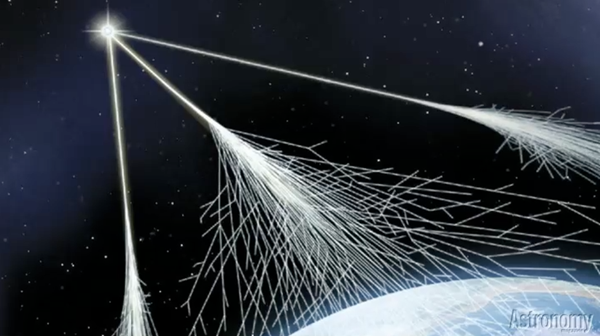
\includegraphics[width = \textwidth]{cosmic}
\caption{The level scheme of $^{135}Pr$ as given in. Clearly labeled are the Yrast, wobbling, Dipole and the Signature partner bands.}
\end{center}
\end{figure}

Cosmic rays are immensely high-energy radiation, mainly originating outside the Solar System. They may produce showers of particles that penetrate and impact the Earth’s atmosphere and sometimes even 
reach the surface. Cosmic rays are composed primarily of protons and alpha particles (99\%), with a small amount of heavier nuclei ($\sim$1\%). When cosmic rays enter the Earth’s atmosphere they collide with atoms and molecules, mainly oxygen and nitrogen. This interaction produces a cascade of lighter particles that rains down on everything on the surface of the Earth.

The exposure received by Cosmic radiation differs for different regions depending upon their elevation. The average dose as received from from cosmic radiation is 0.04 rem per year. 

\end{section}

\begin{section}{Terrestrial Radiation}
\begin{figure}
\begin{center}

\includegraphics[width = 0.5\textwidth]{earth}
\caption{The level scheme of $^{135}Pr$ as given in. Clearly labeled are the Yrast, wobbling, Dipole and the Signature partner bands.}
\end{center}
\end{figure}

The Earth that we live on is in itself a source of radiation. Radioactive materials like Uranium, Thorium and their decay products occur naturally in rocks, soil, water and vegetation. The most harmful of all these decay products is Radon. Radon is a gas and can be inhaled. On reaching our lungs, Radon further decays to solid daughter products that can get stuck in the respiratory system causing harm.

The exposure received by Terrestrial radiation also differs for different parts of the world depending upon the uranium/thorium content of the soil of that area. The average dose from terrestrial radiation is 0.2 rem per year. 

\end{section}

\begin{section}{Internal Radiation}
\begin{figure}
\begin{center}

\includegraphics[width = 0.5\textwidth]{internal_radiation}
\caption{The level scheme of $^{135}Pr$ as given in. Clearly labeled are the Yrast, wobbling, Dipole and the Signature partner bands.}
\end{center}
\end{figure}

All living beings on Earth have Potassium-40, Carbon-14 and Lead-210 in them from the time of their birth. These may arise due to the consumption of food, drinking water or simply inhaling air containing radioactive elements. These elements are absorbed by the tissues and bones in our bodies and keep getting replenished over time by simple processes like ingestion and inhalation.

The exposure received by an average man in the United States by Internal radiation is an effective dose of about 0.03 rem each year.

\end{section}


Transitioning into the man-made sources of radiation, the following can be considered as mostly contributing to the exposure that the general public might receive:

\begin{section}{Medical Procedures}
\begin{figure}
\begin{center}
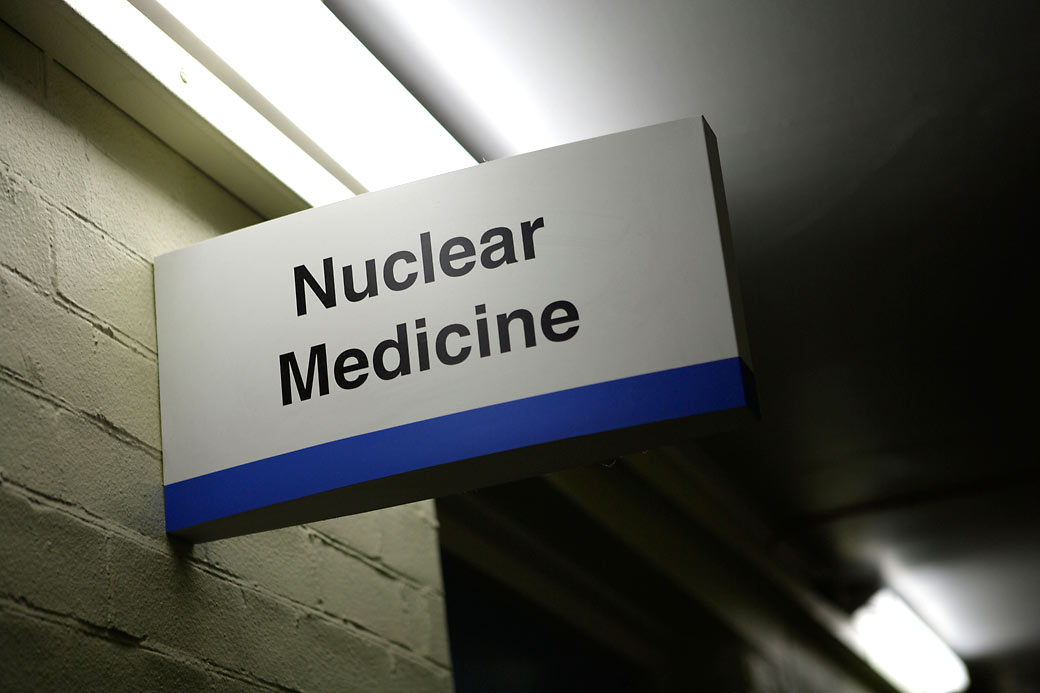
\includegraphics[width = \textwidth]{nuclear-med}
\caption{The level scheme of $^{135}Pr$ as given in. Clearly labeled are the Yrast, wobbling, Dipole and the Signature partner bands.}
\end{center}
\end{figure}

The most radiation exposure as received by the general public from man-made sources, at present is by medical procedures such as X-rays, radiation therapy to cure cancer and medical imaging wherein a radioactive material is injected in the body to check for various diseases. Any patient undergoing such a procedure will receive a radiation dose. The radiation doses delivered to a patient in such an investigation is generally accepted to present a very small risk of inducing cancer. For eg, the effective doses can range from 0.6 mrem to 3.7 rem for a non-specific tumor imaging procedure. A typical chest X-ray can expose you to about 2 mrem of radiation dose while a chest CT-scan can result in up to a dose of 0.2 rem.

\end{section}

\begin{section}{Consumer Products} 
\begin{figure}
\begin{center}
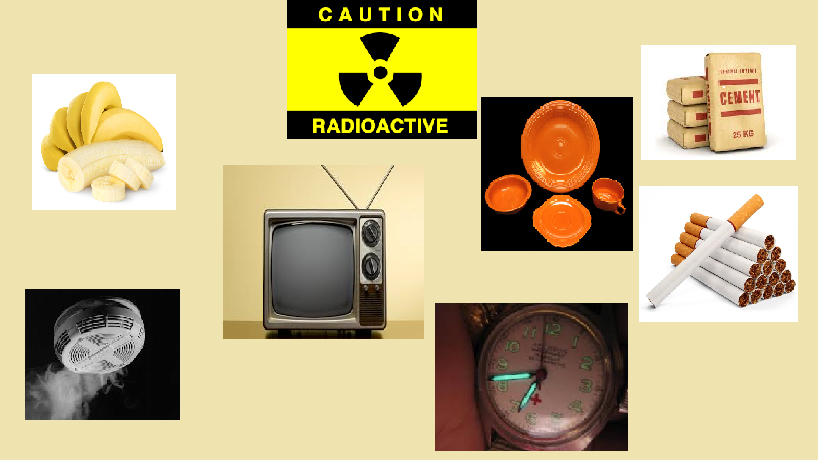
\includegraphics[width = \textwidth]{radiation_household}
\caption{The level scheme of $^{135}Pr$ as given in. Clearly labeled are the Yrast, wobbling, Dipole and the Signature partner bands.}
\end{center}
\end{figure}

Seemingly weird, but if you had a banana this morning, you got yourself exposed to radioactivity. A typical banana contains about half a gram of potassium. That amounts to about an activity of roughly 15 Bq.  Various consumer products that we use in our everyday life, expose us to radiation of different kinds. For example, a smoke detector installed in your house exposes you to about 0.008 mrem of radiation dose per unit. Living in a concrete building will add about 7 mrem per year to your cumulative dose. If you were born before 1972 and ever used the orange-red colored fiesta ware, it must be brought to your notice that back in the day, that special orange-red color was derived from Uranium oxide. Researchers estimate that one such plate would have contained approximately about 4.5 grams of uranium. That being said, if you ate off that dinnerware daily, you would have almost 0.21 grams of uranium ingested per year. But not to worry, fiestaware manufactured after 1972 is not radioactive. But there are plenty of other things that still expose you to a lot of radiation. Tobacco, for instance, due to its property of absorbing radioactive Radon from the atmosphere, will add up to about 1300 mrem per year to your total absorbed dose. 

\end{section}

\begin{section}{Nuclear Fuel Cycle}
\begin{figure}
\begin{center}
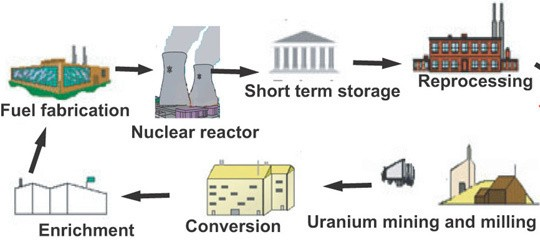
\includegraphics[width = \textwidth]{nuke-cycle}
\caption{The level scheme of $^{135}Pr$ as given in. Clearly labeled are the Yrast, wobbling, Dipole and the Signature partner bands.}
\end{center}
\end{figure}

Surprisingly enough, the source that everyone is most scared of is in fact the least contributing factor  of all the sources of radiation seen so far.  The entire procedure involved in a Nuclear fuel cycle, right from the mining of Uranium to power production exposes the general public to a much lesser radiation dose. To be specific, the average dose equivalent to the US population from the fuel cycle is only about 0.05 mrem per year which is much less than the dose received by any of the natural sources of radiation. It is also much less than any consumer products that we have just seen and of course much much less than what typical X-rays or CT-scans expose you to. 

\end{section}

Just some time back, I came across this wonderful application on the U.S.NRC (United States Nuclear Regulatory Commission) website. The NRC is an independent agency of the US. Government that looks after and protects the public health and safety related to Nuclear energy. This application, also called, Personal Annual Radiation Dose Calculator, allows you to convert your fear factor into an actual number by answering a few simple questions. This number is the total annual radiation dose that you have received depending on where you live, your lifestyle and adds that to the average background radiation that you are ought to receive on Earth. The calculated number has units of mrem (millirem). I got too excited and immediately ended up calculating my annual radiation dose. Here is a screenshot of my result:

\begin{figure}
\begin{center}
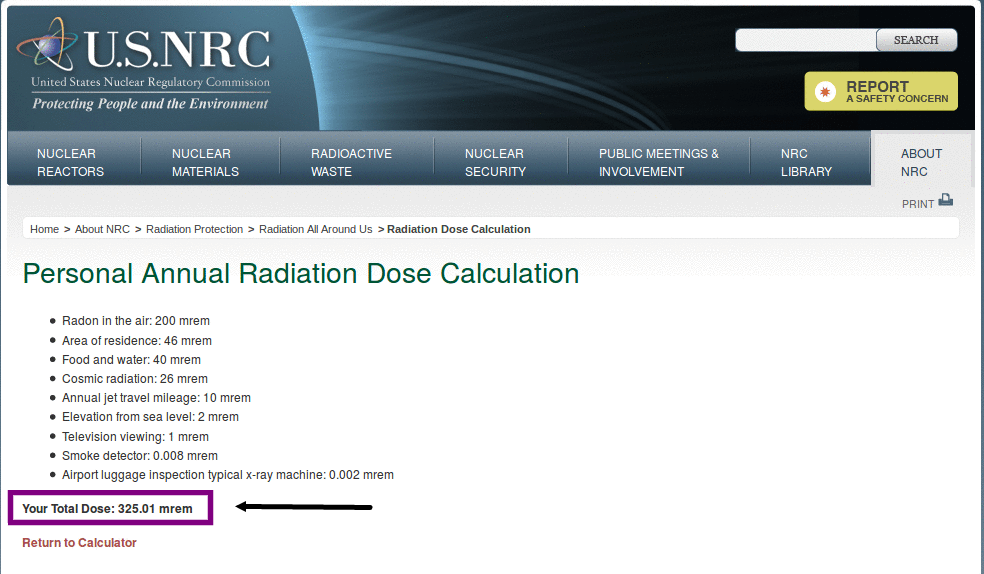
\includegraphics[width = \textwidth]{my_dose}
\caption{The level scheme of $^{135}Pr$ as given in. Clearly labeled are the Yrast, wobbling, Dipole and the Signature partner bands.}
\end{center}
\end{figure}

So my personal dose came out to be 325.01 mrem which is less than the annual average dose per person from all natural and man-made sources of about 350 mrem. Of course, if you have undergone a medical procedure lately, you dose will come out to be a greater number. But the point here is that you don’t have to be living near a nuclear power plant or you don’t have to be working as a Uranium miner  to receive a radiation dose. This calculator, more than anything, makes clear that everyone living on this planet receives a radiation dose, albeit the number might vary depending on your lifestyle and other natural factors.

Another very interesting thought that I came across on the same web page goes something like this;

\textit{“The reduction in life expectancy from a dose of 1 mrem is about 1.2 minutes. This is equivalent to the reduction in life expectancy from crossing the street three times, taking three puffs on a cigarette, or consuming 10 extra calories (for a person who is overweight).”}
 
I am sure everyone reading this is as excited as I was when I first came across this application so here is the link to the web page: 

Calculate your personal annual radiation dose: 

https://www.nrc.gov/about-nrc/radiation/around-us/calculator.html

\end{document}

